\documentclass[a4paper]{article}
\usepackage[top=2cm, bottom=2cm, left=2cm, right=4.5cm, columnsep=1cm]{geometry}
\usepackage{multicol}
\usepackage{graphicx}
\usepackage{rotating}
\usepackage{fancyhdr}
\usepackage[explicit]{titlesec}
\usepackage{enumitem}
\usepackage{hyperref}
\usepackage{helvet}
\usepackage{parskip}
\usepackage{fontspec}
\usepackage[dvipsnames]{xcolor}

\title{\textbf{Galaxy Cube}}
\author{Suricube}
\date{}

% Font for bottom text ------------------------------------------------
\newcommand{\myFontSize}{\fontfamily{phv}\fontseries{l}\fontsize{7.5}{8}\selectfont}
% ----------------------------------------------------------------------

% Suricube Header and Footer --------------------------------------------
\fancypagestyle{datasheet}{
    \fancyhf{} % Clear header and footer
    \renewcommand{\headrulewidth}{0pt} % Remove header rule
    \fancyfoot[L]{\myFontSize\setlength{\parindent}{0pt}Commerzbank Heidelberg · IBAN DE61 6724 0039 0190 2840 00 · BIC COBADEFFXXX St.-Nr. 32498/77488\\
SURICUBE GmbH· Sitz Heidelberg · Amtsgericht Mannheim· HRB 734816 · GF.: Dr. Martin Haas } % Footer content
}
% ----------------------------------------------------------------------

% Suricube Sidebar -----------------------------------------------------
\newcommand{\SuricubeSidebar}{
\marginpar{
  \begin{minipage}{3.8cm}
    
\includegraphics[width=3.8cm]{img/suricube.PNG}
  \end{minipage}
  \begin{turn}{90}
    \begin{minipage}[c][3.8cm]{9.2cm}      
      \fontfamily{phv}\fontseries{l}\fontsize{52}{48}\selectfont SURICUBE
    \end{minipage}
  \end{turn}
  \begin{minipage}[t]{0.2\textwidth}
  \vspace{2cm}
  \begin{flushright}
        \myFontSize
        SURICUBE GmbH\\
        Meyerhofstraße 1 \\ 
        69117 Heidelberg\\
            \vspace{0.2cm}
        T +49 6221 387-8301\\
        F +49 6221 387-897\\
            \vspace{0.2cm}
        info@suricube.de\\
        suricube.de\\
        \end{flushright}
    \end{minipage}
}
}
% ----------------------------------------------------------------------

% Title ---------------------------------------------------------------
\titleformat{name=\section, numberless}[block]
  {\normalfont\fontsize{30}{22}\bfseries}
  {}
  {0pt}
  {#1}
  %{\titlerule[0.5pt]\vspace{0.5ex}\filleft}
  [\titleline{\titlerule[0.1pt]}]
\titlespacing{name=\section, numberless}
  {0pt}
  {2ex}
  {3ex}
% ---------------------------------------------------------------------- 

% Formatting commands for the Section (actually subsections)------------
\titleformat{name=\subsection, numberless}[block]
  {\normalfont\fontsize{14}{16}\bfseries}
  {}
  {0pt}
  {#1}
% ---------------------------------------------------------------------- 

% Remove section numbering----------------------------------------------
\setcounter{secnumdepth}{0}
% ---------------------------------------------------------------------- 

% Lists ----------------------------------------
\setlist[itemize]{label={}, leftmargin=0pt} % Remove bullet points and leftmargin
% ---------------------------------------------------------------------- 

% Custom pandoc command ------------------------------------------------
\providecommand{\tightlist}{\setlength{\itemsep}{0pt}\setlength{\parskip}{0pt}}
% ---------------------------------------------------------------------- 

\begin{document}

\thispagestyle{datasheet}       % Apply Header and Footer
\section*{Galaxy Cube \\        % Title
{\small\color{Gray} Pre-release version}}   % Subtitle
\SuricubeSidebar                % Add Suricube's sidebar
\fontsize{11}{14}\selectfont % Default font for the text body

\begin{minipage}{1\textwidth}
    \begin{multicols}{2}

    % Product picture ----------------------------
    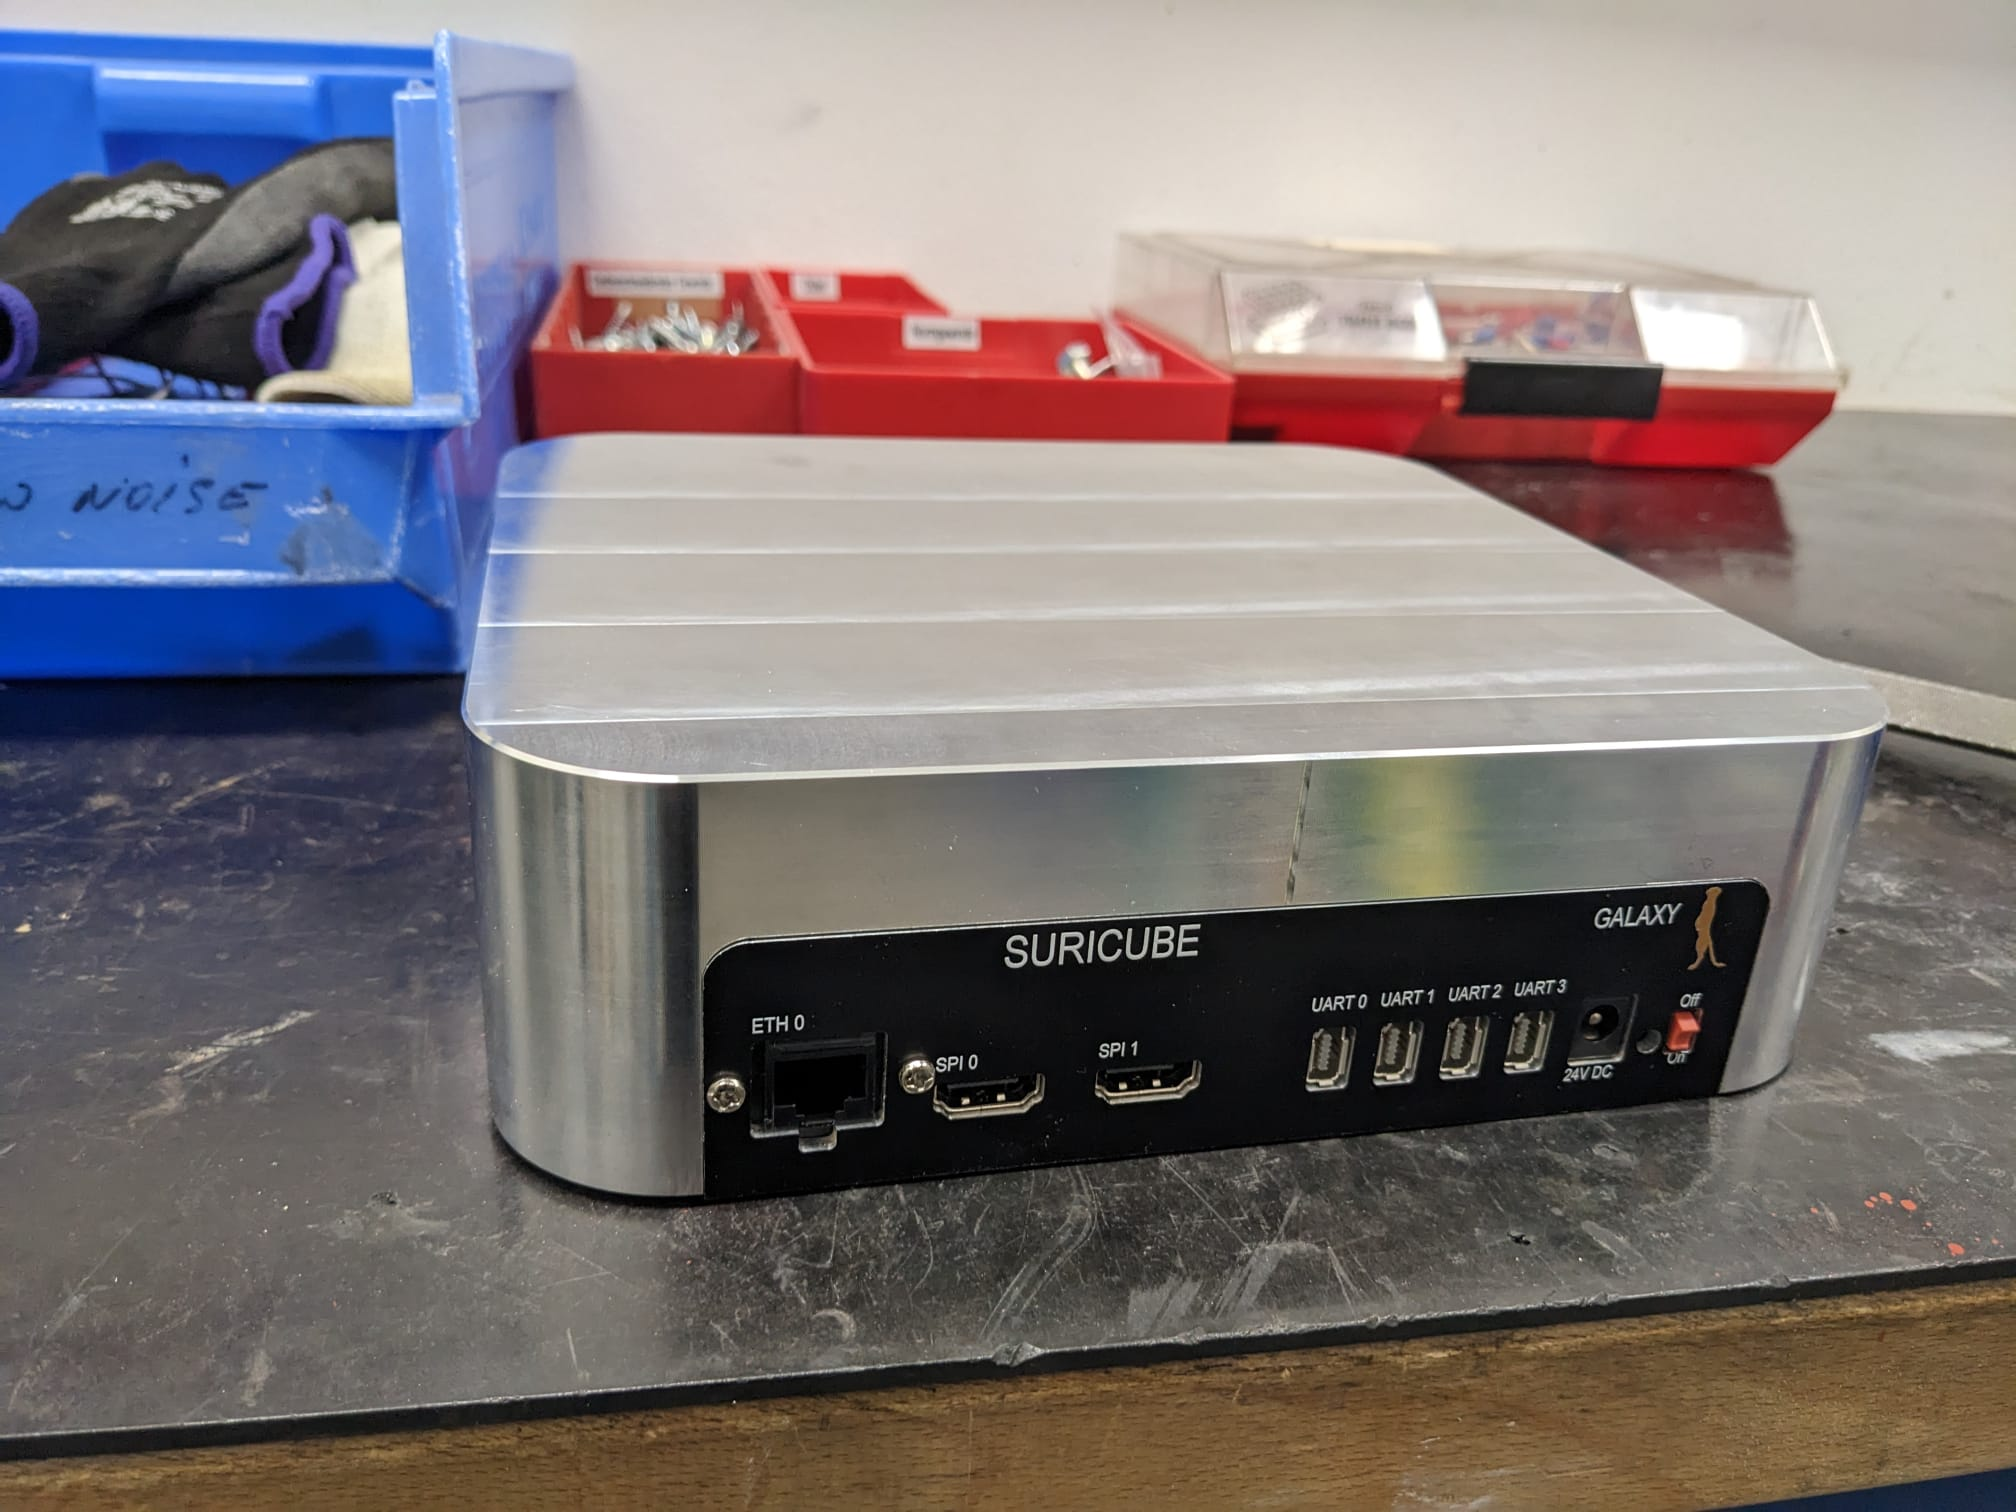
\includegraphics[width=\columnwidth]{img/cube.jpeg} % move to Markdown ?

    % Product Features ----------------------------
    \subsection{Features}\label{features}
        \textbf{ \begin{itemize}
            \tightlist
           \item
              4 high-speed analog outputs
            \item
              8 low-speed analog outputs
            \item
              16 digital input/outputs
            \item
              Arbitrary synchronous waveforms
            \item
              Ethernet communication
        \end{itemize}
        }
    \end{multicols}
\end{minipage}

\vspace{1.0cm}

\begin{multicols}{2}
\hypertarget{general-description}{%
\subsection{General Description}\label{general-description}}

The Galaxy Cube is a microscopy hardware controller. Thanks to its
arbitrary analog output, it can create the needed waveforms for any
device controlled by analog signals, like galvo mirrors. The digital
outputs create trigger lines for laser, camera or other
digitally-controlled devices.

Communication to and from the Galaxy Cube is done through a local
network. Simply connect the Cube to the same network as your
workstation! With a web browser, you can use the Cube for simple
use-cases without need to code anything. For higher modularity needs, an
MQTT-based API is accessible, allowing to integrate all the
functionalities of the Cube into your existing setup.

\hypertarget{product-highlights}{%
\subsection{Product Highlights}\label{product-highlights}}

\hypertarget{high-speed-analog-output}{%
\subsubsection{High-speed analog
output}\label{high-speed-analog-output}}

\begin{itemize}
\tightlist
\item
  Update rate : 1 MHz
\item
  Voltage range : -5V to +5V.
\item
  Settling time : \textasciitilde100ns
\item
  Able to generate arbitrary functions.
\item
  \textit{Can be used to control galvo mirrors.}
\end{itemize}

\hypertarget{low-speed-analog-output}{%
\subsubsection{Low-speed analog output}\label{low-speed-analog-output}}

\begin{itemize}
\tightlist
\item
  Update rate : 50 kHz
\item
  Voltage range : 0 to +5V
\item
  Settling time : 2.5 us (typical)
\item
  \textit{Used for Laser/LED intensity,etc}
\end{itemize}

\hypertarget{digital-i-o-s}{%
\subsubsection{ Digital I/Os}\label{digital-i-o-s}}
\begin{itemize}
\tightlist
\item
  Update rate : 50 MHz
\item
  Logic level : 3.3V
\item
  \textit{Used to get and send trigger signals.}
\end{itemize}

\hypertarget{easy-integration}{%
\subsubsection{Easy integration}\label{easy-integration}}

\begin{itemize}
\tightlist
\item
  Internal Web server for WebUI
\item
  Internal MQTT broker
\item
  Easy-to-use API
\end{itemize}

\end{multicols}

\end{document}